%%%%%%%%%%%%%%%%%%%%%%%%%%%%%%%%%%%%%%%%%%%%%%%%%%%%%%%%%%%%%%%%%%%%%%%%%%%%%%%%
% Template for USENIX papers.
%
% History:
%
% - TEMPLATE for Usenix papers, specifically to meet requirements of
%   USENIX '05. originally a template for producing IEEE-format
%   articles using LaTeX. written by Matthew Ward, CS Department,
%   Worcester Polytechnic Institute. adapted by David Beazley for his
%   excellent SWIG paper in Proceedings, Tcl 96. turned into a
%   smartass generic template by De Clarke, with thanks to both the
%   above pioneers. Use at your own risk. Complaints to /dev/null.
%   Make it two column with no page numbering, default is 10 point.
%
% - Munged by Fred Douglis <douglis@research.att.com> 10/97 to
%   separate the .sty file from the LaTeX source template, so that
%   people can more easily include the .sty file into an existing
%   document. Also changed to more closely follow the style guidelines
%   as represented by the Word sample file.
%
% - Note that since 2010, USENIX does not require endnotes. If you
%   want foot of page notes, don't include the endnotes package in the
%   usepackage command, below.
% - This version uses the latex2e styles, not the very ancient 2.09
%   stuff.
%
% - Updated July 2018: Text block size changed from 6.5" to 7"
%
% - Updated Dec 2018 for ATC'19:
%
%   * Revised text to pass HotCRP's auto-formatting check, with
%     hotcrp.settings.submission_form.body_font_size=10pt, and
%     hotcrp.settings.submission_form.line_height=12pt
%
%   * Switched from \endnote-s to \footnote-s to match Usenix's policy.
%
%   * \section* => \begin{abstract} ... \end{abstract}
%
%   * Make template self-contained in terms of bibtex entires, to allow
%     this file to be compiled. (And changing refs style to 'plain'.)
%
%   * Make template self-contained in terms of figures, to
%     allow this file to be compiled. 
%
%   * Added packages for hyperref, embedding fonts, and improving
%     appearance.
%   
%   * Removed outdated text.
%
%%%%%%%%%%%%%%%%%%%%%%%%%%%%%%%%%%%%%%%%%%%%%%%%%%%%%%%%%%%%%%%%%%%%%%%%%%%%%%%%

\documentclass[letterpaper,twocolumn,10pt]{article}
\usepackage{usenix2019_v3}

% to be able to draw some self-contained figs
\usepackage{tikz}
\usepackage{amsmath}

% inlined bib file
\usepackage{filecontents}
\raggedbottom

\usepackage{graphicx}
\usepackage{float}
\graphicspath{ {../images/}}

%-------------------------------------------------------------------------------
\begin{filecontents}{\jobname.bib}
%-------------------------------------------------------------------------------

\end{filecontents}

%-------------------------------------------------------------------------------
\begin{document}
%-------------------------------------------------------------------------------

%don't want date printed
\date{}

% make title bold and 14 pt font (Latex default is non-bold, 16 pt)
\title{\Large \bf The RISC Takers:\\
  Final Report}

%for single author (just remove % characters)
\author{
  {\rm Sean Keever} \\
  swkeever@uw.edu
  \and
  {\rm Yokesh Jayakumar} \\
  karthj@uw.edu
  \and
  {\rm John McMahon} \\
  mcmahjoh@uw.edu
  % copy the following lines to add more authors
  % \and
  % {\rm Name}\\
  %Name Institution
} % end author

\maketitle

%-------------------------------------------------------------------------------
\begin{abstract}
  %-------------------------------------------------------------------------------
  The goal of our project is to create a means of letting a user not only use an OS,
  but to allow a user to see what is going on inside the OS and CPU.
  To this end, our project aims to maximize availability to users by
  providing a browser-based interface that lets the user visit a webpage and
  visualize an OS from the moment he or she visits the page. We hope that this project
  can grow to be an invaluable teaching tool for instructors, engineers, or anyone.
\end{abstract}

%-------------------------------------------------------------------------------
\section{Introduction}
%-------------------------------------------------------------------------------

There are multiple implementations of operating systems made available via a web
browser. Instead of re-implementing that functionality, we chose to find a project that
has the low-level emulation from C to JavaScript already handled. This way, we can
focus on solving a new problem: providing an interface to
visualize the OS and CPU.

We looked at multiple different OS implementations and decided on riscv-angel,
which seemed to offer the
functionality we needed without too much underlying complexity. This way, we could
focus more attention to creating the visualization layers without having to worry
too much about the low-level emulation details.

%-------------------------------------------------------------------------------
\section{Initial Design}
%-------------------------------------------------------------------------------

To start, we stripped the riscv-angel project to only show the Terminal.
We got rid of all the elements and libraries that were not going to be used in our project.
Before we started on our implementation, we prototyped the UI in Figma, shown in Figure 1.

\begin{figure}[H]
  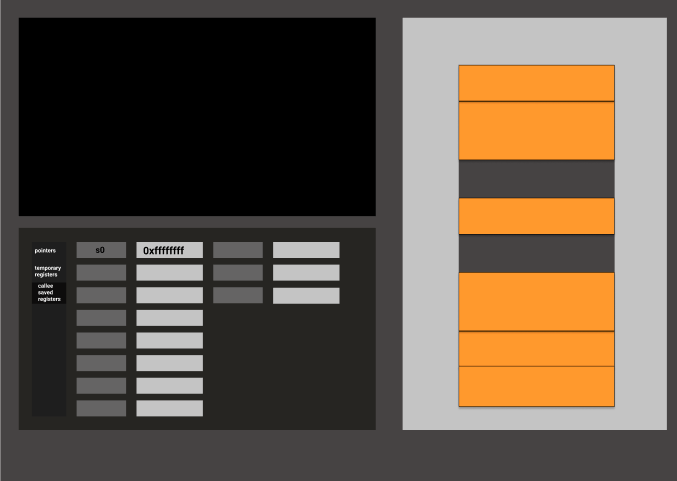
\includegraphics[scale=0.4]{prototype1}
  \caption{Initial prototype of design}
  \label{fig:proto1}
  \centering
\end{figure}

Figma allowed us to come up with a design before we implement anything in code.
We aimed for a dashboard-like interface, showing the user
information about the CPU and OS in real-time. The dashboard interface would
allow the user to have all the information at his fingertips without
having to constantly type commands to get the same information.

%-------------------------------------------------------------------------------
\section{Beginning Development}
%-------------------------------------------------------------------------------

\subsection*{Setting up a development environment}

One of the challenges for the team was facing ambiguity in this project.
It was difficult to interpret exactly what needed to be done.

To facilitate this problem and make development easier,
we started approaching the project with an Agile workflow.
We are using GitHub's Kanban board functionality to track issues and milestones.
We hold weekly stand-ups to find out

\begin{itemize}
  \item what we did over the past week, and
  \item what we will do in the next week.
\end{itemize}

\noindent
We use the GitHub issues that we created to assign tasks for each member of a group.
In doing this, we were able to be more productive by having concrete milestones in place
in order to complete the project.

To ensure robustness and quality of our project,
we have also developed some tooling for continuous integration.
To ensure consistency in the codebase, we use ESLint, a tool that we have configured
to apply the rules defined in AirBnB's style guide.
We use \texttt{lint-staged} to run our linters before any commit. This way,
we know if stylistic errors need to be addressed before pushing code to the repository.

We also set up GitHub Actions, which are essentially hooks that execute when
code is pushed to the repository.
These hooks will run the style checker and our unit tests before code is pushed to remote.
The hook will reject any commits if any of these actions fail.
The GitHub Actions are certainly overkill for our case, but we wanted to have the infrastructure
in place in order to configure our CI easily.

\subsection*{Choosing technologies}

We want our interface to be interactive, so we chose React.js as our library of choice,
which offers a means of rapidly developing interactive client-side applications. React's
rendering mechanism allows for changes in state to immediately update on the browser,
which allowed us to quickly create interactive UI components.

This doesn't come without its challenges, though. The existing project uses vanilla JavaScript
in order to run the emulator. The legacy code accomplishes this by spawning a worker thread
that handles all the emulation tasks. The main thread interacts with this worker thread via
message passing. We will go into more detail about how this message passing functions.

Working with the existing riscv-angel codebase was challenging. We resolved
the issues by having rendering each dashboard component separately. This way,
the dashboard components can coexist with the existing riscv-angel project code
easily. This allowed members to develop features in parallel, without being blocked
by another person's pending change.


%-------------------------------------------------------------------------------
\section{Establishing a Design System}
%-------------------------------------------------------------------------------

None of the members on our team are trained designers. We had to be resourceful
to learn some of the patterns of good UI design. To make this easier, we took
a lot of inspiration from professionals by using the \href{https://material.io/design}{Material Design}
system used and maintained at Google. We imported a Material Design kit into Figma,
which includes many Material Design assets such as buttons, cards, etc. Doing so
allowed us to wireframe a UI prototype that we feel was closer to our vision for the app's design.
Figure \ref{fig:proto2} shows the first steps of prototyping our UI using Material Design and Figma.

\begin{figure}[H]
  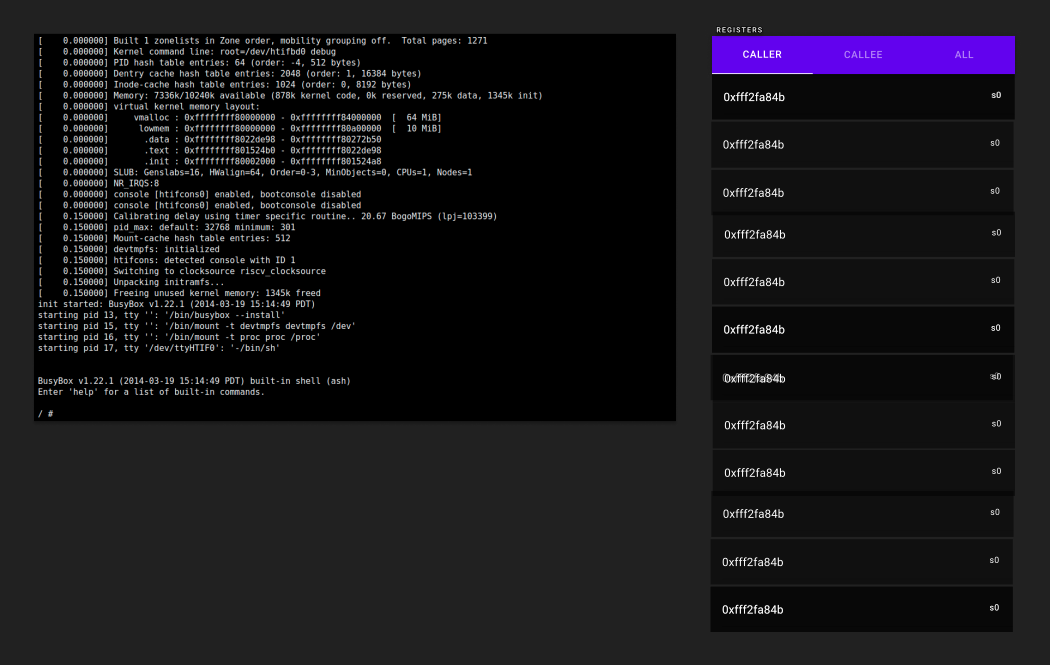
\includegraphics[scale=0.26]{prototype2}
  \caption{Initial prototype using Material Design}
  \label{fig:proto2}
  \centering
\end{figure}

In addition to our team not being expert designers, we are also not experts in CSS, which
is vital to making the application look good. We wanted our application to be as
lightweight as possible, so we wanted to have our own custom CSS, as opposed to using a CSS
framework like Bootstrap. To learn CSS and UI design
patterns further, we read the book \href{https://refactoringui.com/}{Refactoring UI}, which
provided many design tips from a developer's point of view.

We established a design system that is used throughout the app. We defined a system for colors,
fonts, spacing/font size, and more. The system restricts properties of the UI to follow a discrete
set of values. Although at first glance, it may seem that this restriction would limit our ability
to create a design. In fact, the restriction provided by the design system helped to make
the application feel polished and consistent.


%-------------------------------------------------------------------------------
\section{Implementing a Working Prototype}
%-------------------------------------------------------------------------------

\subsection*{A Modular Design}

We describe our app as a modular, dashboard user interface that lets users use a
basic OS and see properties about the OS and CPU in real time.

Our modular design means we have separate components for each visualization in the dashboard.
For example, there is a separate component for the window showing the registers, a separate
component for the view showing the ratio of instructions being executed, and so forth.
\pagebreak
We split our app into modular components for several reasons:

\begin{itemize}
  \item easier to maintain and test
  \item allows features to rapidly developed
  \item offers more flexibility in UI structure
\end{itemize}

We will elaborate on each of these points.

First, because our dashboard interface uses modular UI components, whenever we work on a single
component, we can be confident that breaking a single component won't break other parts of the app.

The modular design also allows us to split the work and develop features independently. This is great for
us during these times of quarantine because of COVID-19. So, for example, while one team member is working on some feature
$A$, another team member can be styling feature $B$. And since the components are modular, we can do so without
worrying about conflicting with another person's work.

Finally, having the components act as modular entities allows us to change the layout of the UI very easily should
we choose too. The components are independent building blocks that can be moved around as we please.
Component independence is very useful for debugging purposes as well, as if one specific component isn't behaving
as intended, then a developer can isolate the problem to that component alone. This
flexibility will become very important when it comes time to finalizing our app.

\subsection*{Finishing our Prototype}

There are two key files in the vanilla Javascript files that direct boot-up. \texttt{boot.js} is run on start-up
of the app and spawns a Webworker (\texttt{webworker.js}), which is a thread that will be running code given to it. This Webworker
thread is in charge of actually computing instructions that will be passed in by \texttt{boot.js}. Once \texttt{boot.js}
passes an insruction, \texttt{webworker.js} will load that instruction and execute it. It will then send the results of that
instruction as a string to \texttt{boot.js}, which will then display the reuslts in the terminal.

This exchange between \texttt{webworker.js} and \texttt{boot.js} is an example of how we use message passing
to pass data between what's shown on the terminal and what is being run in the cpu. Message passing
will be the core method of how results from running instructions will be displayed on the webpage.

Information about the CPU state lives in the existing \texttt{riscv-angel} code, which is written in
vanilla JavaScript. We bind a JavaScript object from the
\texttt{riscv-angel} code
to the globally accessible \texttt{window} object.
To be specific, \texttt{webworker.js} will send the state of the cpu to \texttt{boot.js}, which then binds that cpu state
to the Window object, named as myCpu, which is globally accessible by the React code.
We then create a custom React hook that safely retrieves this state to be used by React.
To further optimize this message passing, \texttt{webworker.js} will only send a cpu state object to \texttt{boot.js}
when the user is interacting with the terminal. If the terminal is idle, then no message will be passed.
This is important to the speed and efficiency of our application, so that it is not slowed down
by constant message passing when it doesn't have to happen.
With the state of the CPU accessible in our React components, we could implement our
dashboard.

In our app, we show the contents of the 32 user registers, the ratio of CPU instructions executed,
and a time series graph showing memory utilization. These are expressed as React components that are
stored in RegisterPanel.js, InstructionPanel.js, and MemoryPanel.js. On boot-up, the application
runs index.js, which renders each of the above components. First we will look at the register panel.

% change this when we have a picture of the prototype
\begin{figure}[H]
  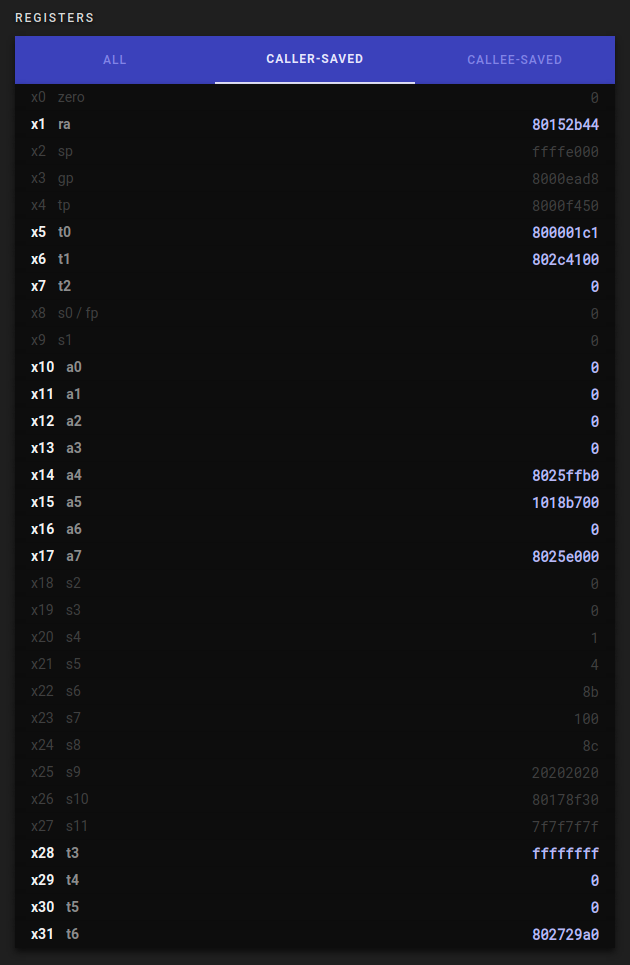
\includegraphics[scale=.35]{reg}
  \label{fig:reg}
  \caption{Register panel}
  \centering
\end{figure}

\noindent

As Figure 3 shows, the register panel shows the:
\begin{itemize}
  \item register name
  \item ABI name
  \item state of each register
\end{itemize}
where the register value will be displayed in 64bit unsigned hexadecimal.
\newpage
We partition the registers into three categories:
\begin{itemize}
  \item all
  \item callee-saved
  \item caller-saved
\end{itemize}

The React hook use-cpu will query for the latest cpu state from the Window object, and set the local
cpu state to be equal to it, on an interval. One this new cpu state is fetched into the React scope,
the register panel will re-render, and display the latest state of the registers. The following components
will follow the same pattern of updating.

The register panel is convenient for the user as all the information is contained in one location. The user
is not forced to be in GDB mode and type commands to get the state of each register. When the cpu state changes,
the register panel updates, so the user does not have to re-type his GDB command. The register panel also
allows the user to validate the proper contents of a register. One future improvement idea is to introduce
a GDB mode, where the user can GDB through programs and have relevant information automatically be
shown on the webpage. The user can use our register panel to see the contents of important registers, such
as ra, sp, etc. Finally, the register panel is helpful to a user who may not be in GDB mode as well.
If a user is running a program, the user can can keep track of the stack pointer and make sure it stays
within a relative area, as this could signify that the program is running as intended, and didn't drastically
change as a result of overflow.

% change this when we have a picture of the prototype
\begin{figure}[H]
  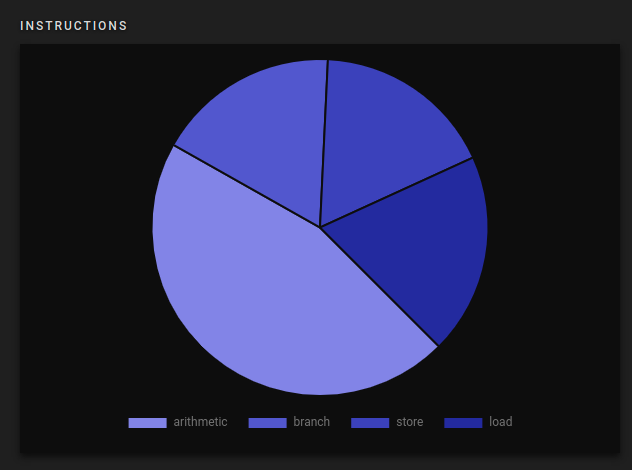
\includegraphics[scale=.4]{inst}
  \label{fig:inst}
  \caption{Instruction panel}
  \centering
\end{figure}

\noindent

Next is the instruction panel shown in Figure 4. The instruction panel shows a running average of four types of instructions:
Arithmetic (ADDI, ANDI, etc), Control Transfer (JAL, JALR), Store (SW, SH, SB, etc), and Load. 
This lets the user see the ratios of each type of instruction and offers 
insight into what's happening beneath the surface. This information can be used by researchers or hardware engineers to
optimize around this ratio. For example, if it looks like arithmetic instructions occur the most often, those developers can design
hardware that prioritizes computation of those instructions over the other types. We actually found that the Memory Ordering 
instructions occured the least, which was always less than 1\% of the total number of instructions being run. Since the ratio
always stayed less than 1\%, we decided to omit graphing this type of instruction usage. Memory Ordering instructions are commonly
used to order device I/O and memory accesses as viewed by hardware threads, and the base linux vm is being run on one process,
which is why this type of instruction is barely used.

% change this when we have a picture of the prototype
\begin{figure}[H]
  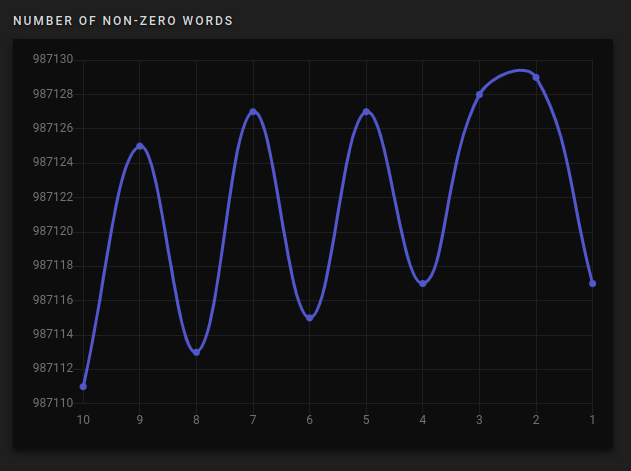
\includegraphics[scale=.4]{mem}
  \label{fig:mem}
  \caption{Memory panel}
  \centering
\end{figure}

\noindent

The memory panel in Figure 5 displays the number of nonzero words in the full memory region and shows the
percentage of words that are not zero. The upper and lower bounds of the graph also dynamically change such that
changes in nonzero word count are visible to the human eye. This is especially evident when the user creates, modifies,
and deletes a file. This graph allows the user to see how much memory has been used, and how much memory is left in
the operating system. This is a useful metric so a user will know if he or she has enough space left to download
a file. As a user uses the terminal to create and edit a file, the upper trend of word usage that will stay constant in
the graph is useful so the user can be aware on-the-fly of how much space is left. Finally, if the user wants to 
attempt a risky deletion process (clearing out many unused directories), the graph will show a steep decline,
as many bytes of memory will clear up on deletion. If the user accidently deletes something without intending to,
this graph's steep drop will alert the user when otherwise the user may not know such deletion ocurred.

We feel that this set of features offers a useful glance at what is going on under the hood
of an operating system utilizing the RISC-V instruction set.

% change this when we have a picture of the prototype
\begin{figure}[H]
  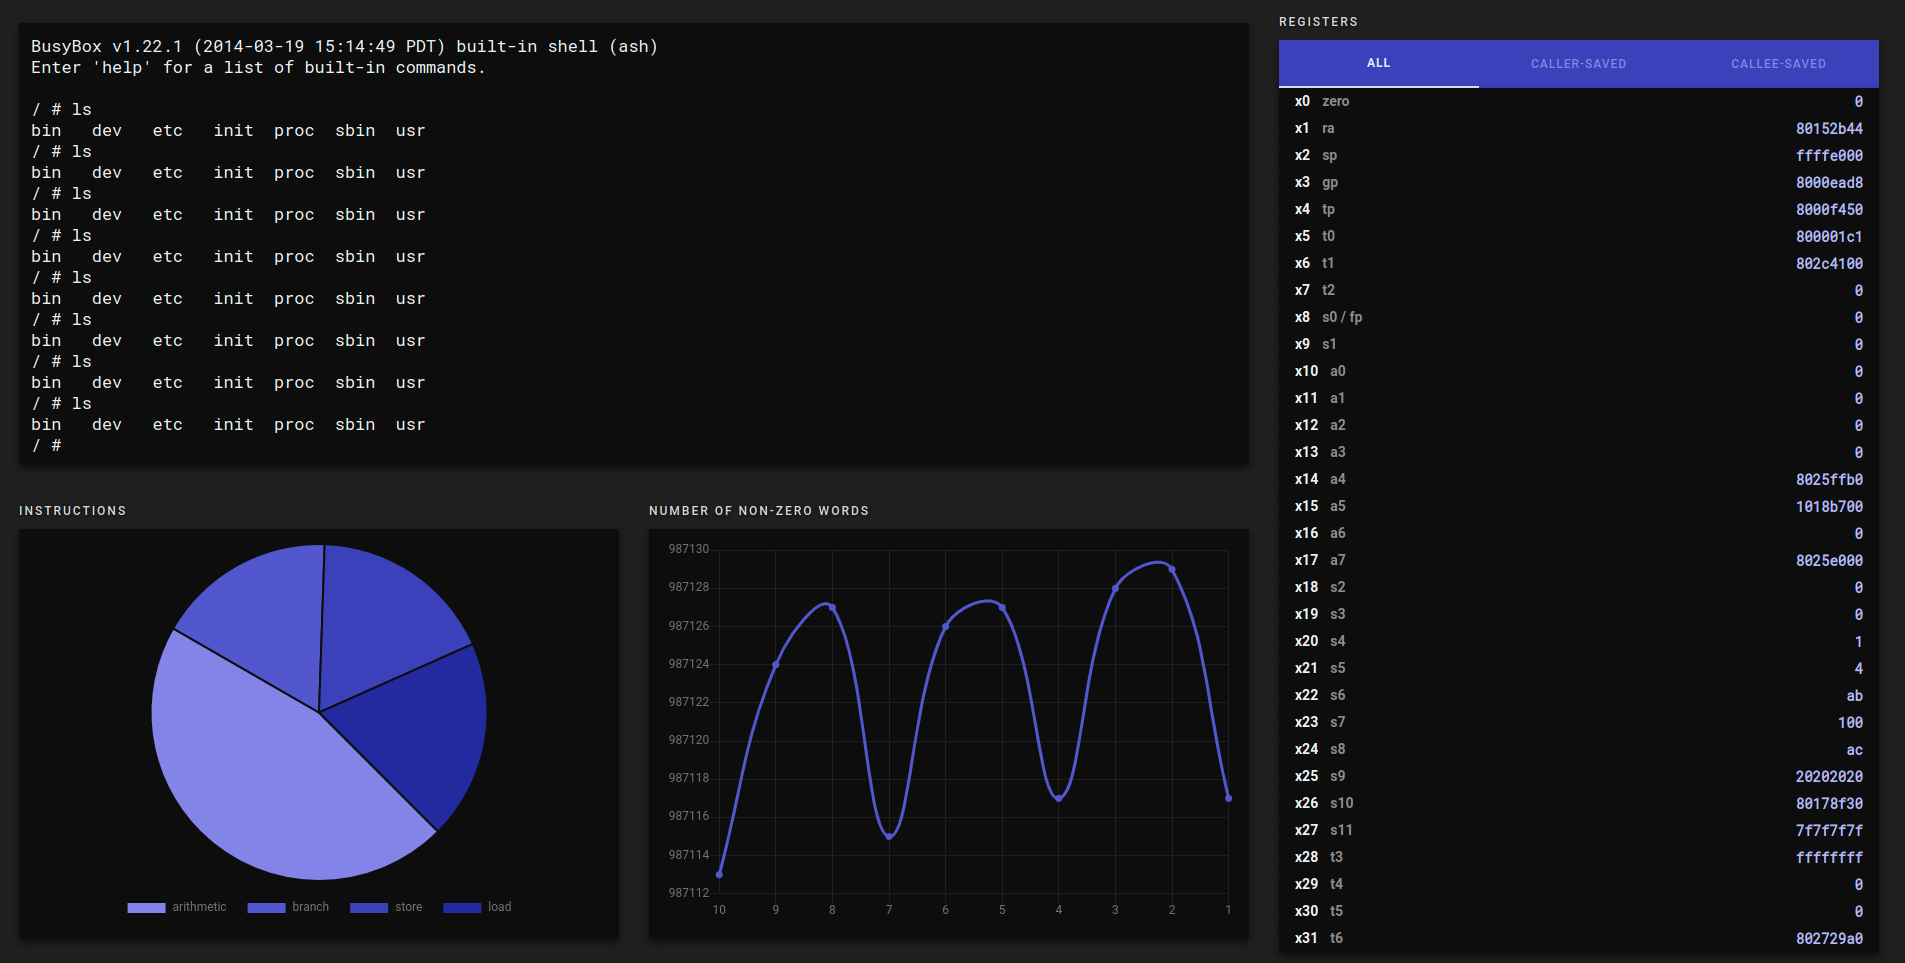
\includegraphics[scale=0.13]{dashboard}
  \label{fig:mvp}
  \caption{MVP}
  \centering
\end{figure}



%-------------------------------------------------------------------------------
\section*{Deployment}
%-------------------------------------------------------------------------------

After our prototype is complete, we prepare our application for deployment.
To keep things as simple as possible, we host the app on the
CSE department's servers at University of Washington. In this way, this project
can easily be used as an example in future iterations of the CSE481a capstone course.


%-------------------------------------------------------------------------------
\section*{Next Steps}
%-------------------------------------------------------------------------------

This project has a lot of room to grow. There are features still to be desired. Namely,

\begin{itemize}
  \item A way to see inside the file system
  \item A way to get information about running processes
  \item An interactive GDB mode
\end{itemize}

One future goal is to bridge the gap between the vanilla Javascript files and our React code.
Instead of message passing the state of the cpu every time there is an update, the ideal architecture
would have the cpu code within the React scope, such as the cpu state changes, it causes
the React components to re-render. Furthermore, if we are able to encompass a given OS binary
into the React scope, a future goal is to allow any OS binary to be swapped with the base
riscv linux vm. This will allow users more flexibility to see metrics on any operating system
of their choosing.

We feel our project provides a modular foundation for these features to be developed in the future.
In hopes to reinvigorate life back into the riscv-angel project, we submitted a pull request
to merge our extensions into the base riscv-angel branch, from which this project is based on.



%-------------------------------------------------------------------------------
\section*{Conclusion}
%-------------------------------------------------------------------------------

In this project, we've taken an existing project, riscv-angel, and extended it to display
an interactive dashboard that lets users see the internals of an OS and CPU running on
a virtual machine.
We believe our project could be used by educators to easily show students properties of
an OS in real time.
We designed and developed this application with modularity in mind.
Our React component-based architecture allows features to rapidly developed and added to the UI.
We believe this application has the potential to reinvigorate interest in the original riscv-angel project.
At the very least, people can use our app to learn and experiment with an operating system running on a RISC-V architecture
with very little barrier to entry.


%-------------------------------------------------------------------------------
\section*{Acknowledgments}
%-------------------------------------------------------------------------------

Thanks to all of the contributors of \href{https://github.com/riscv/riscv-angel}{riscv-angel},
in which this project is based on.

%-------------------------------------------------------------------------------
\section*{Availability}
%-------------------------------------------------------------------------------

This project is open-source and is available at
\href{https://github.com/swkeever/riscv-angel-extended}
{https://github.com/swkeever/riscv-angel-extended}

%-------------------------------------------------------------------------------


%%%%%%%%%%%%%%%%%%%%%%%%%%%%%%%%%%%%%%%%%%%%%%%%%%%%%%%%%%%%%%%%%%%%%%%%%%%%%%%%
\end{document}
%%%%%%%%%%%%%%%%%%%%%%%%%%%%%%%%%%%%%%%%%%%%%%%%%%%%%%%%%%%%%%%%%%%%%%%%%%%%%%%%

%%  LocalWords:  endnotes includegraphics fread ptr nobj noindent
%%  LocalWords:  pdflatex acks
